% !TeX root=../main.tex

\chapter{مقدمه}
% دستور زیر باعث عدم‌نمایش شماره صفحه در اولین صفحهٔ این فصل می‌شود.
%\thispagestyle{empty}
در این فصل، ابتدا مقدمه‌ای درباره‌ی تولید انعطاف‌پذیر ارائه شده و به بررسی دلایل استفاده از این روش در صنایع مختلف پرداخته می‌شود. سپس، پس از معرفی فناوری‌های موجود برای پیاده‌سازی این نوع تولید، ویژگی‌ها، مزایا و معایب هر یک به‌صورت جامع ارزیابی می‌گردد. در پایان، با توجه به اهداف این پژوهش، ساختارهای مبتنی بر شناوری مغناطیسی معرفی شده و با توجه به ویژگی‌های منحصربه‌فرد این فناوری، کاربردهای آن در سایر صنایع نیز مورد بحث قرار می‌گیرد.

\section{مقدمه‌ای بر تولید انعطاف‌پذیر}

با رشد صنایع تولیدی مدرن و افزایش تنوع محصولات، خطوط تولید سنتی دیگر نمی‌توانند به سرعت به تغییرات پاسخ دهند. هرگونه تغییر در این خطوط نیازمند جابه‌جایی دستگاه‌ها یا تغییر مسیر نوارهای نقاله است که این کار هزینه‌های زیادی به همراه دارد و به دلیل زمان‌بر بودن و هزینه‌های بالا، اغلب عملی نیست.
\textit{تولید انعطاف‌پذیر} 
به سامانه‌ای از ماشین‌آلات صنعتی اشاره دارد که به‌طور کنترل‌شده قادر به پردازش مقدار متوسطی از محصولات به صورت هم‌زمان هستند
\cite{browne1984classification}.
 این رویکرد با کنار گذاشتن روندهای خطی سنتی و بهره‌گیری از فرایندهای پیچیده‌تر، امکان تولید سریع‌تر را فراهم می‌کند.

یکی از الزامات اصلی برای پیاده‌سازی تولید انعطاف‌پذیر، طراحی جایگزین‌هایی برای نوارهای نقاله است تا کنترل دقیق‌تری بر محصولات در جریان تولید اعمال شود. امکان جابه‌جایی محصولات در دو راستای طولی و عرضی، به‌عنوان نخستین گام در ارتقای خطوط تولید و افزایش انعطاف‌پذیری مطرح است و برای دستیابی به این هدف، روش‌های متعددی ارائه شده است.

یکی از این روش‌ها که در پژوهش‌های مختلف مورد بررسی قرار گرفته، استفاده از چرخ‌های چندجهته است که می‌تواند راهکاری مناسب برای کنترل موقعیت محصولات باشد. در این سازوکار، با تغییر وضعیت چرخ‌های مختلف و تنظیم جهت چرخش آنها، امکان جابه‌جایی محصولات در راستاهای طولی و عرضی، و همچنین چرخش حول محور عمودی فراهم می‌شود که به‌طور مؤثری به افزایش انعطاف‌پذیری خطوط تولید کمک می‌کند.
شکل \ref{fig:flexiblewheel:one}. 
استفاده از ربات‌های چرخ‌دار که قادر به جابه‌جایی در محیط‌های مسطح هستند نیز به‌عنوان یک راهکار برای انتقال محصولات در برخی صنایع معرفی شده است. 
شکل \ref{fig:flexiblewheel:two}.  
با این‌ حال، فناوری‌های مبتنی‌ بر چرخ به‌ دلیل تماس فیزیکی ناگزیر میان محصولات و ماشین‌آلات با محدودیت‌هایی روبه‌رو هستند که استفاده از آن‌ها را در صنایع خاص دشوار می‌کند. یکی از چالش‌های اصلی این روش، وجود اصطکاک میان چرخ‌ها و محصولات است که در گام اول، به‌عنوان عاملی غیرقابل‌ پیش‌بینی در حرکت محصولات عمل کرده و دقت جابه‌جایی را به‌طور چشمگیری کاهش می‌دهد. علاوه‌ بر این، اصطکاک موجود، سرعت و شتاب حرکت محصولات را محدود کرده و از عملکرد بهینه جلوگیری می‌کند.
یکی دیگر از محدودیت‌های سیستم‌های چرخ‌دار، ساختار مکانیکی آن‌ها است که می‌تواند باعث ایجاد گرد و غبار در محیط شود و به همین دلیل در صنایعی که نیاز به فضای بدون آلودگی یا خلاء دارند، نمی‌توان از این فناوری استفاده کرد.

\begin{figure}[ht]
\centering 
\subfloat[استفاده از چرخ های چند جهته]{ \label{fig:flexiblewheel:one}
\includegraphics[width=0.5\textwidth]{cellular1}}
%\hspace{2mm}
\subfloat[استفاده از ربات های چرخ دار]{ \label{fig:flexiblewheel:two}
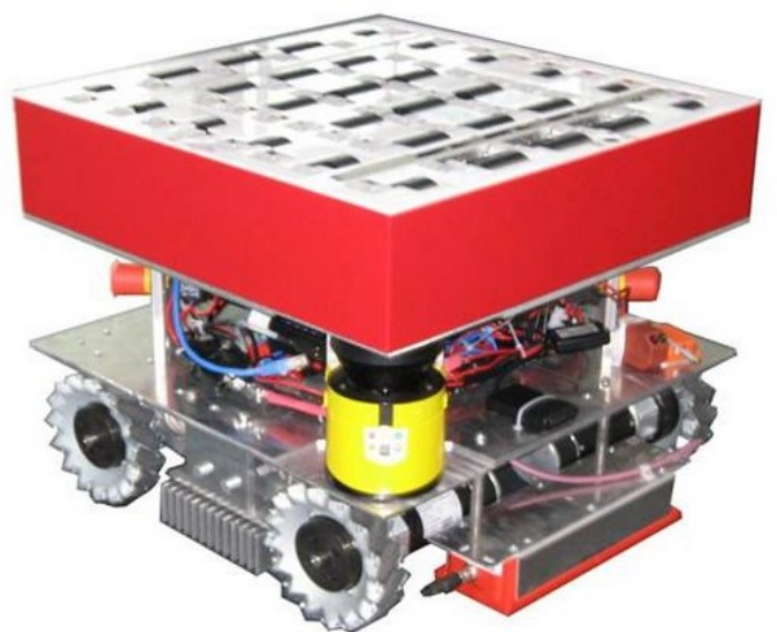
\includegraphics[width=0.5\textwidth]{KARIS}}%
\caption{طراحی های تولید انعطاف پذیر مبتنی بر چرخ}
\label{fig:flexiblewheel} %% label for entire figure
\end{figure}
در مقابل، موتورهای مسطح مبتنی‌ بر شناوری مغناطیسی
\LTRfootnote{Magnetic Levitated Planar Motors (MLPM)}
 توانسته‌اند بسیاری از این محدودیت‌ها را برطرف کنند. با حذف تماس فیزیکی بین محصولات و سطح، نیروی اصطکاک از معادلات حرکت به‌طور کامل حذف می‌شود و این امکان فراهم می‌آید که حرکت محصولات با دقت بسیار بالایی کنترل شود. در این فناوری، نیروی اعمال‌شده به جسم متحرک از طریق میدان‌های مغناطیسی ناشی از جریان الکتریکی در سیم‌پیچ‌ها تولید می‌شود و به همین دلیل، می‌توان با دقت بالایی میزان نیروی واردشده و جابه‌جایی محصول را محاسبه و تنظیم کرد. همچنین این روش برخلاف روش‌های مبتنی‌ بر چرخ، امکان جابه‌جایی محصولات با سرعت و شتاب بالا و بدون ایجاد گرد و غبار را فراهم می‌کند. علاوه‌ بر این، اجزای متحرک در این سامانه‌ها می‌توانند تا شش درجه آزادی داشته باشند و بدون هیچ محدودیتی روی سطح استاتور حرکت کنند.



\section{مقدمه‌ای بر موتورهای مسطح مبتنی‌ بر شناوری مغناطیسی}

شناوری مغناطیسی به معنای اعمال نیروهای مغناطیسی به اجسام به‌گونه‌ای است که این نیروها بتوانند بر نیروی جاذبه غلبه کرده و جسم را بدون تماس فیزیکی و به‌صورت پایدار در هوا معلق نگه ‌دارند. این نیرو می‌تواند به دو شکل جاذبه یا دافعه اعمال شود. در حالت جاذبه‌، نیروی مغناطیسی از بالا به جسم وارد شده و نیروی گرانش زمین را خنثی می‌کند، درحالی‌ که در حالت دافعه، نیرو از پایین به جسم وارد شده و آن را به سمت بالا دفع می‌کند. در صورتی‌که جسم فقط دارای خاصیت رسانایی باشد، تنها امکان جذب‌شدن وجود دارد، اما اگر جسم از مواد مغناطیسی مانند آهنرباهای دائمی یا الکتریکی ساخته شود، می‌تواند هم جذب و هم دفع شود.

کنترل نیروهای مغناطیسی معمولاً با استفاده از آهنرباهای الکتریکی انجام می‌شود، به‌طوری ‌که عبور جریان الکتریکی از سیم‌پیچ‌ها میدان مغناطیسی ایجاد کرده و تنظیم این جریان‌ها باعث تغییر در شدت میدان و نیروی وارده به جسم می‌شود. از این طریق، می‌توان با کنترل دقیق جریان، جسم را به‌طور پایدار در حالت معلق نگه داشت.

در موتورهای مسطح مبتنی‌ بر شناوری مغناطیسی، نیروی مغناطیسی همواره از بخش زیرین به جسم وارد می‌شود. در این سیستم‌ها، دو نوع طراحی رایج است: 1) آهنرباهای الکتریکی در بخش استاتور قرار می‌گیرند و بخش متحرک از آهنرباهای دائمی ساخته) می‌شود، و یا 2) استاتور شامل آهنرباهای دائمی است و آهنرباهای الکتریکی در بخش متحرک جای می‌گیرند. در هر دو حالت، با تنظیم جریان در سیم‌پیچ‌های بخش متحرک، نیروی اعمالی کنترل شده و حرکت جسم تنظیم می‌شود.

در کاربردهای صنعتی، به‌دلیل نیاز به بازدهی بالاتر در تبدیل انرژی مغناطیسی به نیرو، از آرایه‌های خاصی از آهنرباهای دائمی به نام 
\textit{آرایه هالباخ}
\LTRfootnote{Halbach array}
استفاده می‌شود. این آرایه‌ها به‌گونه‌ای طراحی شده‌اند که میدان مغناطیسی را به‌طور متمرکز در یک سمت تقویت کنند و در نتیجه، نیروی مغناطیسی بیشتری به جسم وارد شود. ساختارهای آرایه هالباخ یک‌بعدی و دوبعدی در تحقیقات پیشین به‌طور گسترده بررسی و استفاده شده‌اند.

برای پیاده‌سازی موفق یک سیستم شناوری مغناطیسی، عوامل متعددی باید در نظر گرفته شوند که شامل طراحی و بهینه‌سازی ساختار مکانیکی سیستم، پیاده‌سازی کنترلرهای دقیق برای تنظیم نیروهای مغناطیسی، و همچنین مدل‌سازی دینامیکی یا شناسایی رفتار سیستم برای کنترل بهتر آن است. این عوامل به‌طور مستقیم بر کارایی و پایداری سیستم تأثیر می‌گذارند و باید به‌دقت مورد بررسی و تنظیم قرار گیرند.

